% Created by tikzDevice version 0.12.6 on 2026-07-03 04:21:20
% !TEX encoding = UTF-8 Unicode
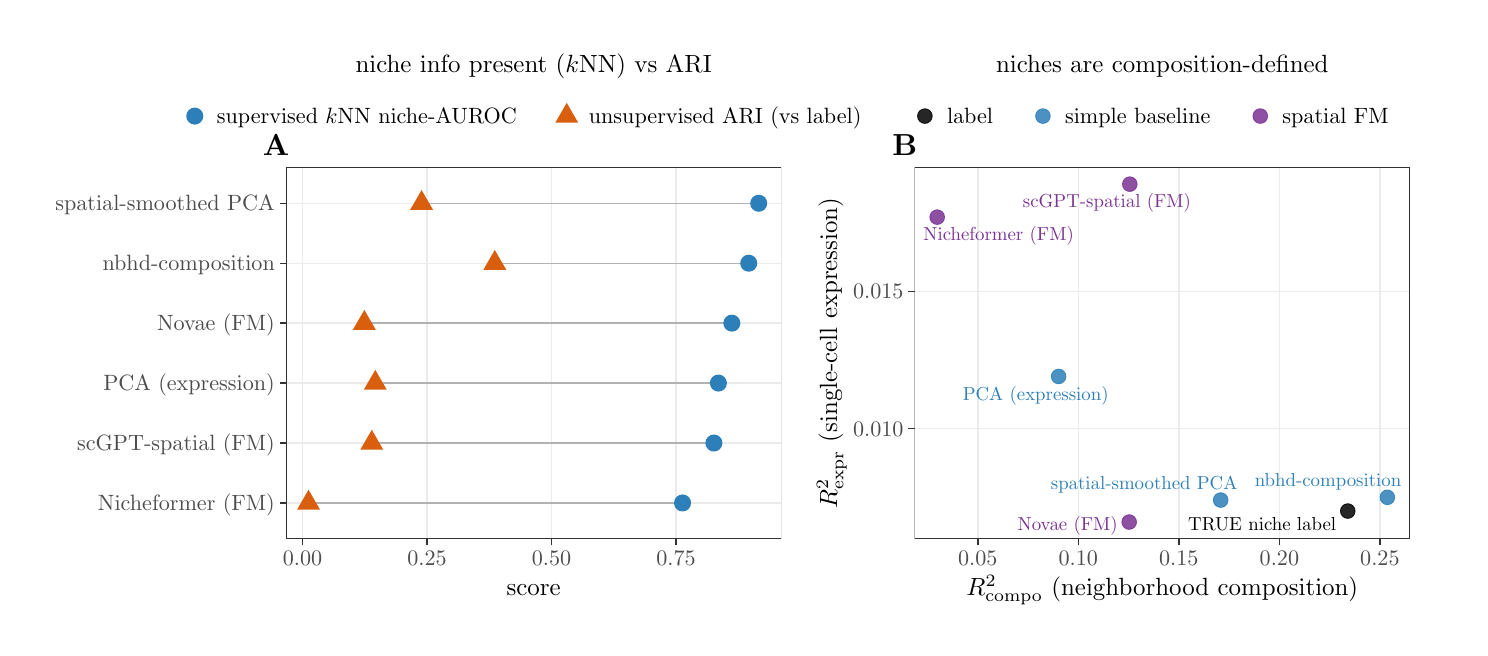
\begin{tikzpicture}[x=1pt,y=1pt]
\definecolor{fillColor}{RGB}{255,255,255}
\path[use as bounding box,fill=fillColor,fill opacity=0.00] (0,0) rectangle (517.45,216.81);
\begin{scope}
\path[clip] (  0.00,  0.00) rectangle (517.45,216.81);
\definecolor{drawColor}{RGB}{255,255,255}
\definecolor{fillColor}{RGB}{255,255,255}

\path[draw=drawColor,line width= 0.5pt,line join=round,line cap=round,fill=fillColor] (  0.00,  0.00) rectangle (517.45,216.81);
\end{scope}
\begin{scope}
\path[clip] (  5.00,  5.00) rectangle (281.30,211.81);
\definecolor{drawColor}{RGB}{255,255,255}
\definecolor{fillColor}{RGB}{255,255,255}

\path[draw=drawColor,line width= 0.5pt,line join=round,line cap=round,fill=fillColor] (  5.00,  5.00) rectangle (281.30,211.81);
\end{scope}
\begin{scope}
\path[clip] (281.30,  5.00) rectangle (508.45,211.81);
\definecolor{drawColor}{RGB}{255,255,255}
\definecolor{fillColor}{RGB}{255,255,255}

\path[draw=drawColor,line width= 0.5pt,line join=round,line cap=round,fill=fillColor] (281.30,  5.00) rectangle (508.45,211.81);
\end{scope}
\begin{scope}
\path[clip] ( 93.36, 32.07) rectangle (272.30,166.36);
\definecolor{fillColor}{RGB}{255,255,255}

\path[fill=fillColor] ( 93.36, 32.07) rectangle (272.30,166.36);
\definecolor{drawColor}{gray}{0.92}

\path[draw=drawColor,line width= 0.5pt,line join=round] ( 93.36, 45.06) --
	(272.30, 45.06);

\path[draw=drawColor,line width= 0.5pt,line join=round] ( 93.36, 66.72) --
	(272.30, 66.72);

\path[draw=drawColor,line width= 0.5pt,line join=round] ( 93.36, 88.38) --
	(272.30, 88.38);

\path[draw=drawColor,line width= 0.5pt,line join=round] ( 93.36,110.04) --
	(272.30,110.04);

\path[draw=drawColor,line width= 0.5pt,line join=round] ( 93.36,131.70) --
	(272.30,131.70);

\path[draw=drawColor,line width= 0.5pt,line join=round] ( 93.36,153.36) --
	(272.30,153.36);

\path[draw=drawColor,line width= 0.5pt,line join=round] ( 99.34, 32.07) --
	( 99.34,166.36);

\path[draw=drawColor,line width= 0.5pt,line join=round] (144.32, 32.07) --
	(144.32,166.36);

\path[draw=drawColor,line width= 0.5pt,line join=round] (189.31, 32.07) --
	(189.31,166.36);

\path[draw=drawColor,line width= 0.5pt,line join=round] (234.29, 32.07) --
	(234.29,166.36);
\definecolor{drawColor}{gray}{0.70}

\path[draw=drawColor,line width= 0.5pt,line join=round] (101.49, 45.06) --
	(236.63, 45.06);

\path[draw=drawColor,line width= 0.5pt,line join=round] (124.35, 66.72) --
	(247.97, 66.72);

\path[draw=drawColor,line width= 0.5pt,line join=round] (125.61, 88.38) --
	(249.59, 88.38);

\path[draw=drawColor,line width= 0.5pt,line join=round] (121.65,110.04) --
	(254.45,110.04);

\path[draw=drawColor,line width= 0.5pt,line join=round] (168.79,131.70) --
	(260.56,131.70);

\path[draw=drawColor,line width= 0.5pt,line join=round] (142.34,153.36) --
	(264.16,153.36);
\definecolor{fillColor}{RGB}{217,95,14}

\path[fill=fillColor] (168.79,136.49) --
	(172.94,129.31) --
	(164.65,129.31) --
	cycle;

\path[fill=fillColor] (125.61, 93.17) --
	(129.75, 85.99) --
	(121.46, 85.99) --
	cycle;

\path[fill=fillColor] (142.34,158.15) --
	(146.48,150.97) --
	(138.20,150.97) --
	cycle;

\path[fill=fillColor] (101.49, 49.85) --
	(105.64, 42.67) --
	( 97.35, 42.67) --
	cycle;

\path[fill=fillColor] (121.65,114.83) --
	(125.79,107.65) --
	(117.51,107.65) --
	cycle;

\path[fill=fillColor] (124.35, 71.51) --
	(128.49, 64.33) --
	(120.21, 64.33) --
	cycle;
\definecolor{fillColor}{RGB}{44,127,184}

\path[fill=fillColor] (260.56,131.70) circle (  3.08);

\path[fill=fillColor] (249.59, 88.38) circle (  3.08);

\path[fill=fillColor] (264.16,153.36) circle (  3.08);

\path[fill=fillColor] (236.63, 45.06) circle (  3.08);

\path[fill=fillColor] (254.45,110.04) circle (  3.08);

\path[fill=fillColor] (247.97, 66.72) circle (  3.08);
\definecolor{drawColor}{gray}{0.20}

\path[draw=drawColor,line width= 0.5pt,line join=round,line cap=round] ( 93.36, 32.07) rectangle (272.30,166.36);
\end{scope}
\begin{scope}
\path[clip] (  0.00,  0.00) rectangle (517.45,216.81);
\definecolor{drawColor}{gray}{0.30}

\node[text=drawColor,anchor=base east,inner sep=0pt, outer sep=0pt, scale=  0.80] at ( 89.31, 42.31) {Nicheformer (FM)};

\node[text=drawColor,anchor=base east,inner sep=0pt, outer sep=0pt, scale=  0.80] at ( 89.31, 63.97) {scGPT-spatial (FM)};

\node[text=drawColor,anchor=base east,inner sep=0pt, outer sep=0pt, scale=  0.80] at ( 89.31, 85.63) {PCA (expression)};

\node[text=drawColor,anchor=base east,inner sep=0pt, outer sep=0pt, scale=  0.80] at ( 89.31,107.29) {Novae (FM)};

\node[text=drawColor,anchor=base east,inner sep=0pt, outer sep=0pt, scale=  0.80] at ( 89.31,128.95) {nbhd-composition};

\node[text=drawColor,anchor=base east,inner sep=0pt, outer sep=0pt, scale=  0.80] at ( 89.31,150.61) {spatial-smoothed PCA};
\end{scope}
\begin{scope}
\path[clip] (  0.00,  0.00) rectangle (517.45,216.81);
\definecolor{drawColor}{gray}{0.20}

\path[draw=drawColor,line width= 0.5pt,line join=round] ( 91.11, 45.06) --
	( 93.36, 45.06);

\path[draw=drawColor,line width= 0.5pt,line join=round] ( 91.11, 66.72) --
	( 93.36, 66.72);

\path[draw=drawColor,line width= 0.5pt,line join=round] ( 91.11, 88.38) --
	( 93.36, 88.38);

\path[draw=drawColor,line width= 0.5pt,line join=round] ( 91.11,110.04) --
	( 93.36,110.04);

\path[draw=drawColor,line width= 0.5pt,line join=round] ( 91.11,131.70) --
	( 93.36,131.70);

\path[draw=drawColor,line width= 0.5pt,line join=round] ( 91.11,153.36) --
	( 93.36,153.36);
\end{scope}
\begin{scope}
\path[clip] (  0.00,  0.00) rectangle (517.45,216.81);
\definecolor{drawColor}{gray}{0.20}

\path[draw=drawColor,line width= 0.5pt,line join=round] ( 99.34, 29.82) --
	( 99.34, 32.07);

\path[draw=drawColor,line width= 0.5pt,line join=round] (144.32, 29.82) --
	(144.32, 32.07);

\path[draw=drawColor,line width= 0.5pt,line join=round] (189.31, 29.82) --
	(189.31, 32.07);

\path[draw=drawColor,line width= 0.5pt,line join=round] (234.29, 29.82) --
	(234.29, 32.07);
\end{scope}
\begin{scope}
\path[clip] (  0.00,  0.00) rectangle (517.45,216.81);
\definecolor{drawColor}{gray}{0.30}

\node[text=drawColor,anchor=base,inner sep=0pt, outer sep=0pt, scale=  0.80] at ( 99.34, 22.51) {0.00};

\node[text=drawColor,anchor=base,inner sep=0pt, outer sep=0pt, scale=  0.80] at (144.32, 22.51) {0.25};

\node[text=drawColor,anchor=base,inner sep=0pt, outer sep=0pt, scale=  0.80] at (189.31, 22.51) {0.50};

\node[text=drawColor,anchor=base,inner sep=0pt, outer sep=0pt, scale=  0.80] at (234.29, 22.51) {0.75};
\end{scope}
\begin{scope}
\path[clip] (  0.00,  0.00) rectangle (517.45,216.81);
\definecolor{drawColor}{RGB}{0,0,0}

\node[text=drawColor,anchor=base,inner sep=0pt, outer sep=0pt, scale=  0.90] at (182.83, 11.75) {score};
\end{scope}
\begin{scope}
\path[clip] (  0.00,  0.00) rectangle (517.45,216.81);
\definecolor{fillColor}{RGB}{255,255,255}

\path[fill=fillColor] ( 50.88,175.36) rectangle (314.78,194.36);
\end{scope}
\begin{scope}
\path[clip] (  0.00,  0.00) rectangle (517.45,216.81);
\definecolor{fillColor}{RGB}{255,255,255}

\path[fill=fillColor] ( 55.38,179.86) rectangle ( 65.38,189.86);
\definecolor{fillColor}{RGB}{44,127,184}

\path[fill=fillColor] ( 60.38,184.86) circle (  3.08);
\end{scope}
\begin{scope}
\path[clip] (  0.00,  0.00) rectangle (517.45,216.81);
\definecolor{fillColor}{RGB}{255,255,255}

\path[fill=fillColor] (189.79,179.86) rectangle (199.79,189.86);
\definecolor{fillColor}{RGB}{217,95,14}

\path[fill=fillColor] (194.79,189.64) --
	(198.93,182.47) --
	(190.65,182.47) --
	cycle;
\end{scope}
\begin{scope}
\path[clip] (  0.00,  0.00) rectangle (517.45,216.81);
\definecolor{drawColor}{RGB}{0,0,0}

\node[text=drawColor,anchor=base west,inner sep=0pt, outer sep=0pt, scale=  0.80] at ( 68.38,182.10) {supervised $k$NN niche-AUROC};
\end{scope}
\begin{scope}
\path[clip] (  0.00,  0.00) rectangle (517.45,216.81);
\definecolor{drawColor}{RGB}{0,0,0}

\node[text=drawColor,anchor=base west,inner sep=0pt, outer sep=0pt, scale=  0.80] at (202.79,182.10) {unsupervised ARI (vs label)};
\end{scope}
\begin{scope}
\path[clip] (  0.00,  0.00) rectangle (517.45,216.81);
\definecolor{drawColor}{RGB}{0,0,0}

\node[text=drawColor,anchor=base,inner sep=0pt, outer sep=0pt, scale=  0.90] at (182.83,200.61) {niche info present ($k$NN) vs ARI};
\end{scope}
\begin{scope}
\path[clip] (  0.00,  0.00) rectangle (517.45,216.81);
\definecolor{drawColor}{RGB}{0,0,0}

\node[text=drawColor,anchor=base,inner sep=0pt, outer sep=0pt, scale=  1.10] at ( 89.78,170.57) {\bfseries A};
\end{scope}
\begin{scope}
\path[clip] (320.52, 32.07) rectangle (499.45,166.36);
\definecolor{fillColor}{RGB}{255,255,255}

\path[fill=fillColor] (320.52, 32.07) rectangle (499.45,166.36);
\definecolor{drawColor}{gray}{0.92}

\path[draw=drawColor,line width= 0.5pt,line join=round] (320.52, 71.92) --
	(499.45, 71.92);

\path[draw=drawColor,line width= 0.5pt,line join=round] (320.52,121.55) --
	(499.45,121.55);

\path[draw=drawColor,line width= 0.5pt,line join=round] (343.33, 32.07) --
	(343.33,166.36);

\path[draw=drawColor,line width= 0.5pt,line join=round] (379.65, 32.07) --
	(379.65,166.36);

\path[draw=drawColor,line width= 0.5pt,line join=round] (415.98, 32.07) --
	(415.98,166.36);

\path[draw=drawColor,line width= 0.5pt,line join=round] (452.31, 32.07) --
	(452.31,166.36);

\path[draw=drawColor,line width= 0.5pt,line join=round] (488.63, 32.07) --
	(488.63,166.36);
\definecolor{drawColor}{RGB}{0,0,0}
\definecolor{fillColor}{RGB}{0,0,0}

\path[draw=drawColor,draw opacity=0.85,line width= 0.3pt,line join=round,line cap=round,fill=fillColor,fill opacity=0.85] (477.01, 42.14) circle (  2.65);
\definecolor{drawColor}{RGB}{44,127,184}
\definecolor{fillColor}{RGB}{44,127,184}

\path[draw=drawColor,draw opacity=0.85,line width= 0.3pt,line join=round,line cap=round,fill=fillColor,fill opacity=0.85] (491.32, 47.10) circle (  2.65);

\path[draw=drawColor,draw opacity=0.85,line width= 0.3pt,line join=round,line cap=round,fill=fillColor,fill opacity=0.85] (372.53, 90.78) circle (  2.65);

\path[draw=drawColor,draw opacity=0.85,line width= 0.3pt,line join=round,line cap=round,fill=fillColor,fill opacity=0.85] (431.09, 46.11) circle (  2.65);
\definecolor{drawColor}{RGB}{123,50,148}
\definecolor{fillColor}{RGB}{123,50,148}

\path[draw=drawColor,draw opacity=0.85,line width= 0.3pt,line join=round,line cap=round,fill=fillColor,fill opacity=0.85] (328.65,148.35) circle (  2.65);

\path[draw=drawColor,draw opacity=0.85,line width= 0.3pt,line join=round,line cap=round,fill=fillColor,fill opacity=0.85] (398.03, 38.17) circle (  2.65);

\path[draw=drawColor,draw opacity=0.85,line width= 0.3pt,line join=round,line cap=round,fill=fillColor,fill opacity=0.85] (398.25,160.26) circle (  2.65);
\definecolor{drawColor}{RGB}{0,0,0}

\node[text=drawColor,anchor=base,inner sep=0pt, outer sep=0pt, scale=  0.68] at (446.09, 35.08) {TRUE niche label};
\definecolor{drawColor}{RGB}{44,127,184}

\node[text=drawColor,anchor=base,inner sep=0pt, outer sep=0pt, scale=  0.68] at (469.87, 50.96) {nbhd-composition};

\node[text=drawColor,anchor=base,inner sep=0pt, outer sep=0pt, scale=  0.68] at (364.26, 82.22) {PCA (expression)};

\node[text=drawColor,anchor=base,inner sep=0pt, outer sep=0pt, scale=  0.68] at (403.43, 49.96) {spatial-smoothed PCA};
\definecolor{drawColor}{RGB}{123,50,148}

\node[text=drawColor,anchor=base,inner sep=0pt, outer sep=0pt, scale=  0.68] at (350.85,139.80) {Nicheformer (FM)};

\node[text=drawColor,anchor=base,inner sep=0pt, outer sep=0pt, scale=  0.68] at (375.81, 35.08) {Novae (FM)};

\node[text=drawColor,anchor=base,inner sep=0pt, outer sep=0pt, scale=  0.68] at (390.01,151.71) {scGPT-spatial (FM)};
\definecolor{drawColor}{gray}{0.20}

\path[draw=drawColor,line width= 0.5pt,line join=round,line cap=round] (320.52, 32.07) rectangle (499.45,166.36);
\end{scope}
\begin{scope}
\path[clip] (  0.00,  0.00) rectangle (517.45,216.81);
\definecolor{drawColor}{gray}{0.30}

\node[text=drawColor,anchor=base east,inner sep=0pt, outer sep=0pt, scale=  0.80] at (316.47, 69.16) {0.010};

\node[text=drawColor,anchor=base east,inner sep=0pt, outer sep=0pt, scale=  0.80] at (316.47,118.79) {0.015};
\end{scope}
\begin{scope}
\path[clip] (  0.00,  0.00) rectangle (517.45,216.81);
\definecolor{drawColor}{gray}{0.20}

\path[draw=drawColor,line width= 0.5pt,line join=round] (318.27, 71.92) --
	(320.52, 71.92);

\path[draw=drawColor,line width= 0.5pt,line join=round] (318.27,121.55) --
	(320.52,121.55);
\end{scope}
\begin{scope}
\path[clip] (  0.00,  0.00) rectangle (517.45,216.81);
\definecolor{drawColor}{gray}{0.20}

\path[draw=drawColor,line width= 0.5pt,line join=round] (343.33, 29.82) --
	(343.33, 32.07);

\path[draw=drawColor,line width= 0.5pt,line join=round] (379.65, 29.82) --
	(379.65, 32.07);

\path[draw=drawColor,line width= 0.5pt,line join=round] (415.98, 29.82) --
	(415.98, 32.07);

\path[draw=drawColor,line width= 0.5pt,line join=round] (452.31, 29.82) --
	(452.31, 32.07);

\path[draw=drawColor,line width= 0.5pt,line join=round] (488.63, 29.82) --
	(488.63, 32.07);
\end{scope}
\begin{scope}
\path[clip] (  0.00,  0.00) rectangle (517.45,216.81);
\definecolor{drawColor}{gray}{0.30}

\node[text=drawColor,anchor=base,inner sep=0pt, outer sep=0pt, scale=  0.80] at (343.33, 22.51) {0.05};

\node[text=drawColor,anchor=base,inner sep=0pt, outer sep=0pt, scale=  0.80] at (379.65, 22.51) {0.10};

\node[text=drawColor,anchor=base,inner sep=0pt, outer sep=0pt, scale=  0.80] at (415.98, 22.51) {0.15};

\node[text=drawColor,anchor=base,inner sep=0pt, outer sep=0pt, scale=  0.80] at (452.31, 22.51) {0.20};

\node[text=drawColor,anchor=base,inner sep=0pt, outer sep=0pt, scale=  0.80] at (488.63, 22.51) {0.25};
\end{scope}
\begin{scope}
\path[clip] (  0.00,  0.00) rectangle (517.45,216.81);
\definecolor{drawColor}{RGB}{0,0,0}

\node[text=drawColor,anchor=base,inner sep=0pt, outer sep=0pt, scale=  0.90] at (409.99, 11.75) {$R^2_{\mathrm{compo}}$ (neighborhood composition)};
\end{scope}
\begin{scope}
\path[clip] (  0.00,  0.00) rectangle (517.45,216.81);
\definecolor{drawColor}{RGB}{0,0,0}

\node[text=drawColor,rotate= 90.00,anchor=base,inner sep=0pt, outer sep=0pt, scale=  0.90] at (292.50, 99.21) {$R^2_{\mathrm{expr}}$ (single-cell expression)};
\end{scope}
\begin{scope}
\path[clip] (  0.00,  0.00) rectangle (517.45,216.81);
\definecolor{fillColor}{RGB}{255,255,255}

\path[fill=fillColor] (314.70,175.36) rectangle (505.27,194.36);
\end{scope}
\begin{scope}
\path[clip] (  0.00,  0.00) rectangle (517.45,216.81);
\definecolor{fillColor}{RGB}{255,255,255}

\path[fill=fillColor] (319.20,179.86) rectangle (329.20,189.86);
\definecolor{drawColor}{RGB}{0,0,0}
\definecolor{fillColor}{RGB}{0,0,0}

\path[draw=drawColor,draw opacity=0.85,line width= 0.3pt,line join=round,line cap=round,fill=fillColor,fill opacity=0.85] (324.20,184.86) circle (  2.65);
\end{scope}
\begin{scope}
\path[clip] (  0.00,  0.00) rectangle (517.45,216.81);
\definecolor{fillColor}{RGB}{255,255,255}

\path[fill=fillColor] (361.86,179.86) rectangle (371.86,189.86);
\definecolor{drawColor}{RGB}{44,127,184}
\definecolor{fillColor}{RGB}{44,127,184}

\path[draw=drawColor,draw opacity=0.85,line width= 0.3pt,line join=round,line cap=round,fill=fillColor,fill opacity=0.85] (366.86,184.86) circle (  2.65);
\end{scope}
\begin{scope}
\path[clip] (  0.00,  0.00) rectangle (517.45,216.81);
\definecolor{fillColor}{RGB}{255,255,255}

\path[fill=fillColor] (440.40,179.86) rectangle (450.40,189.86);
\definecolor{drawColor}{RGB}{123,50,148}
\definecolor{fillColor}{RGB}{123,50,148}

\path[draw=drawColor,draw opacity=0.85,line width= 0.3pt,line join=round,line cap=round,fill=fillColor,fill opacity=0.85] (445.40,184.86) circle (  2.65);
\end{scope}
\begin{scope}
\path[clip] (  0.00,  0.00) rectangle (517.45,216.81);
\definecolor{drawColor}{RGB}{0,0,0}

\node[text=drawColor,anchor=base west,inner sep=0pt, outer sep=0pt, scale=  0.80] at (332.20,182.10) {label};
\end{scope}
\begin{scope}
\path[clip] (  0.00,  0.00) rectangle (517.45,216.81);
\definecolor{drawColor}{RGB}{0,0,0}

\node[text=drawColor,anchor=base west,inner sep=0pt, outer sep=0pt, scale=  0.80] at (374.86,182.10) {simple baseline};
\end{scope}
\begin{scope}
\path[clip] (  0.00,  0.00) rectangle (517.45,216.81);
\definecolor{drawColor}{RGB}{0,0,0}

\node[text=drawColor,anchor=base west,inner sep=0pt, outer sep=0pt, scale=  0.80] at (453.40,182.10) {spatial FM};
\end{scope}
\begin{scope}
\path[clip] (  0.00,  0.00) rectangle (517.45,216.81);
\definecolor{drawColor}{RGB}{0,0,0}

\node[text=drawColor,anchor=base,inner sep=0pt, outer sep=0pt, scale=  0.90] at (409.99,200.61) {niches are composition-defined};
\end{scope}
\begin{scope}
\path[clip] (  0.00,  0.00) rectangle (517.45,216.81);
\definecolor{drawColor}{RGB}{0,0,0}

\node[text=drawColor,anchor=base,inner sep=0pt, outer sep=0pt, scale=  1.10] at (316.94,170.57) {\bfseries B};
\end{scope}
\end{tikzpicture}
